\documentclass[a4paper]{article}

%% Language and font encodings
\usepackage[english]{babel}
\usepackage[utf8x]{inputenc}
\usepackage[T1]{fontenc}

%% Sets page size and margins
\usepackage[a4paper,top=3cm,bottom=2cm,left=3cm,right=3cm,marginparwidth=1.75cm]{geometry}

%% Useful packages
\usepackage{amsmath}
\usepackage{graphicx}
\usepackage[colorinlistoftodos]{todonotes}

\usepackage{indentfirst}

%% reference
\usepackage{natbib}
\usepackage{hyperref}
\hypersetup{
     colorlinks   = true,
     linkcolor    = red,
     citecolor    = blue
}

\title{\bf Hierarchical Topic Models and the Nested Chinese Restaurant Process}
\author{Tun-Chieh Hsu, Xialingzi Jin,Yen-Hua Chen}

\begin{document}
\maketitle



\section{Abstract}


\section{Background}

The paper we selected is Hierarchical Topic Models and the Nested Chinese Restaurant Process \cite{Blei_Griffiths_Jordan_Tenenbaum_2004}. 

Recently, complex probabilistic models are increasingly prevalent in various of  domains. However, there are several challenges that should be dealt with due to their open-ended nature. That is, the data sets often grow over time, as they growing, they bring new entities and new structures to the fore. Take the problem of learning a topic hierarchy from data for example. Given a collection of ``documents'', each of which contains a set of ``words'' and the goal is to discover common usage patterns or ``topics'' in the documents, and to organize these topics into a hierarchy. 


This paper proposes a new method that specified a generative probabilistic model
for hierarchical structures and adopt Bayesian perspective to learn such structures from data. 
The hierarchies in this case could be considered as random variables and specified procedurally.
In addition, the underlying approach of constructing the probabilistic object is Chinese restaurant process (CRP), a distribution on partitions of integers. In this paper, they extend CRP to a hierarchy of partitions and apply it as a representation of prior and posterior distributions for topic hierarchies. To be more specific, each node in the hierarchy is associated with a topic, where a topic is a distribution across words. A document is generated by choosing a path from the root to a leaf, repeatedly sampling topics along that path, and sampling the words from the selected topics. Thus the organization of topics into a hierarchy aims to capture the breadth of usage of topics across the corpus, reflecting underlying syntactic and semantic notions of generality and specificity. 

There are several approaches to the modeling of topic hierarchies in the literatures. Most of them were constructed on the hypothesis that the distributions between leaf and root are similar. This approach, however, does not based on such constraint.

\section{Algorithm Description}
In order to introduce this method, we should first introduce the Chinese restaurant process (CRP). 
\subsection{The Chinese restaurant process}

CRP is an analogous to seating customers at tables in a Chinese restaurant. Imagine there is a Chinese restaurant with an infinite number of circular tables, each with infinite capacity. Customer 1 sits at the first table. The next customer either sits at the same table as customer 1, or the next table.  The $mth$ subsequent customer sits at a table drawn from the following
distribution: 

\begin{align}
p(\text{occupied table i| previous customers}) =  \frac{m_i}{\gamma+m-1}  \\ 
p(\text{next unoccupied table | previous customers}) = \frac{\gamma}{\gamma + m -1} &
\end{align}

where $m_i$ is the number of previous customers at table $i$, and $\gamma$ is a parameter. After $M$
customers sit down, the seating plan gives a partition of $M$ items. This distribution gives
the same partition structure as draws from a Dirichlet process.

\subsection{Nested Chinese restaurant process}

A nested Chinese restaurant process (nCRP) is an extended version of CRP. Suppose that there are an infinite number of infinite-table Chinese restaurants in a city. And restaurant is determined to be the root restaurant and on each of its infinite tables is a card
with the name of another restaurant. On each of the tables in those restaurants are cards that
refer to other restaurants, and this structure repeats infinitely. Each restaurant is referred to
exactly once. As a result, the whole process could be imagined as an infinitely-branched tree. Now, consider 
a tourist arrives in the city for a culinary vacation. On the first first day, he select a root
Chinese restaurant and selects a table from the equation above. On the second day, he enters to the
restaurant refered by previous restaurant , again from the above equation.
This process was repeated for $L$ days, and at the end, the tourist has sat at L restaurants
which constitute a path from the root to a restaurant at the $L$th level in the infinite tree
After M tourists take L-day vacations, the collection of paths describe a
particular L-level subtree of the infinite tree.

\subsection{A hierarchical topic model}

The hierarchical latent Dirichlet allocation model (hLDA) together with nested Chinese restaruant process (nCRP) illustrate the pattern of {\it words} from the collection of {\it documents}. There are 3 procedures in hLDA: (1) Draw a path from root-node to a leaf; (2) Select a specific path, draw a vector of topic along the path; (3) Draw the words from the topic.

\begin{itemize}
\setlength{\itemsep}{0pt}
\setlength{\parsep}{0pt}
\setlength{\parskip}{0pt}
\item [1.] Let $c_{1}$ be the root restaurant.
\item [2.] For each level $\ell\in\{2,...,L\}$:
	\begin{itemize}
	\item [(a)] Draw a table from restaurant $c_{\ell-1}$ using CRP. Set $c_{\ell}$ to be the restaurant reffered to by that table.
	\end{itemize}
\item [3.] Draw an $L$-dimensional topic proportion vector $\theta$ from Dir$(\alpha)$.
\item [4.] For each word $n\in\{1,...,N\}$:
	\begin{itemize}
	\item [(a)] Draw $z\in\{1,...,L\}$ from Mult$(\theta)$.
	\item [(b)] Draw $w_{n}$ from the topic associated with restaurant $c_{z}$.
	\end{itemize}
\end{itemize}

\begin{figure}
\center
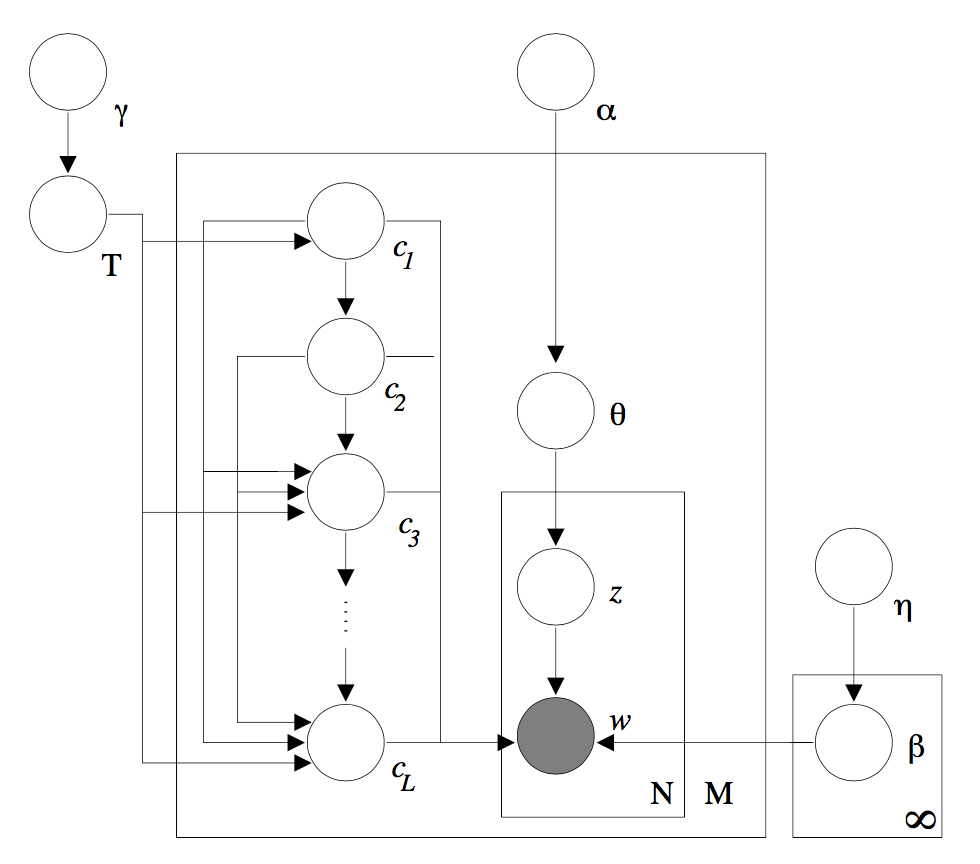
\includegraphics[width=0.5\textwidth]{hLDA.png}
\caption{ The graphical model representation of hierarchical LDA with a
nested CRP prior}
\label{fig:mesh1}
\end{figure}


\subsection{Approximate Inference by Gibbs Sampling}
We then can approximate infer by Gibbs sampling by 2 parts: (1) sample the $z_{m,n}$, the assignment of $n$th word in the $m$th document to the one of the topics $z\in\{1,...,L\}$\cite{Griffiths_Steyvers_2002}; (2) sample the $c_{m}$, the restaurant (topic) corresponding to the $\ell$th topic in document $m$.


\begin{align}
p(z_{i}=j|\mathbf{z}_{-i},\mathbf{w})&\propto\frac{n_{-i,j}^{(w_{i})}+\beta}{n_{-i,j}^{(\cdot)}+W\beta}\frac{n_{-i,j}^{(d_{i})}+\alpha}{n_{-i,\cdot}^{(d_{i})}+T\alpha}\\
p(\mathbf{c}_{m}|\mathbf{w},\mathbf{c}_{-m},\mathbf{z})&\propto p(\mathbf{w}_{m}|\mathbf{c},\mathbf{w}_{-m},\mathbf{z})p(\mathbf{c}_{m}|\mathbf{c}_{-m})
\end{align}


\section{Applications to simulated data sets}

In this section, we apply hLDA on the simulated data. The data included 10 documents with 10 words in each document.  In the experiments, we let the sampler burn in for 10000 iterations and control the level. 

\begin{figure}
\center
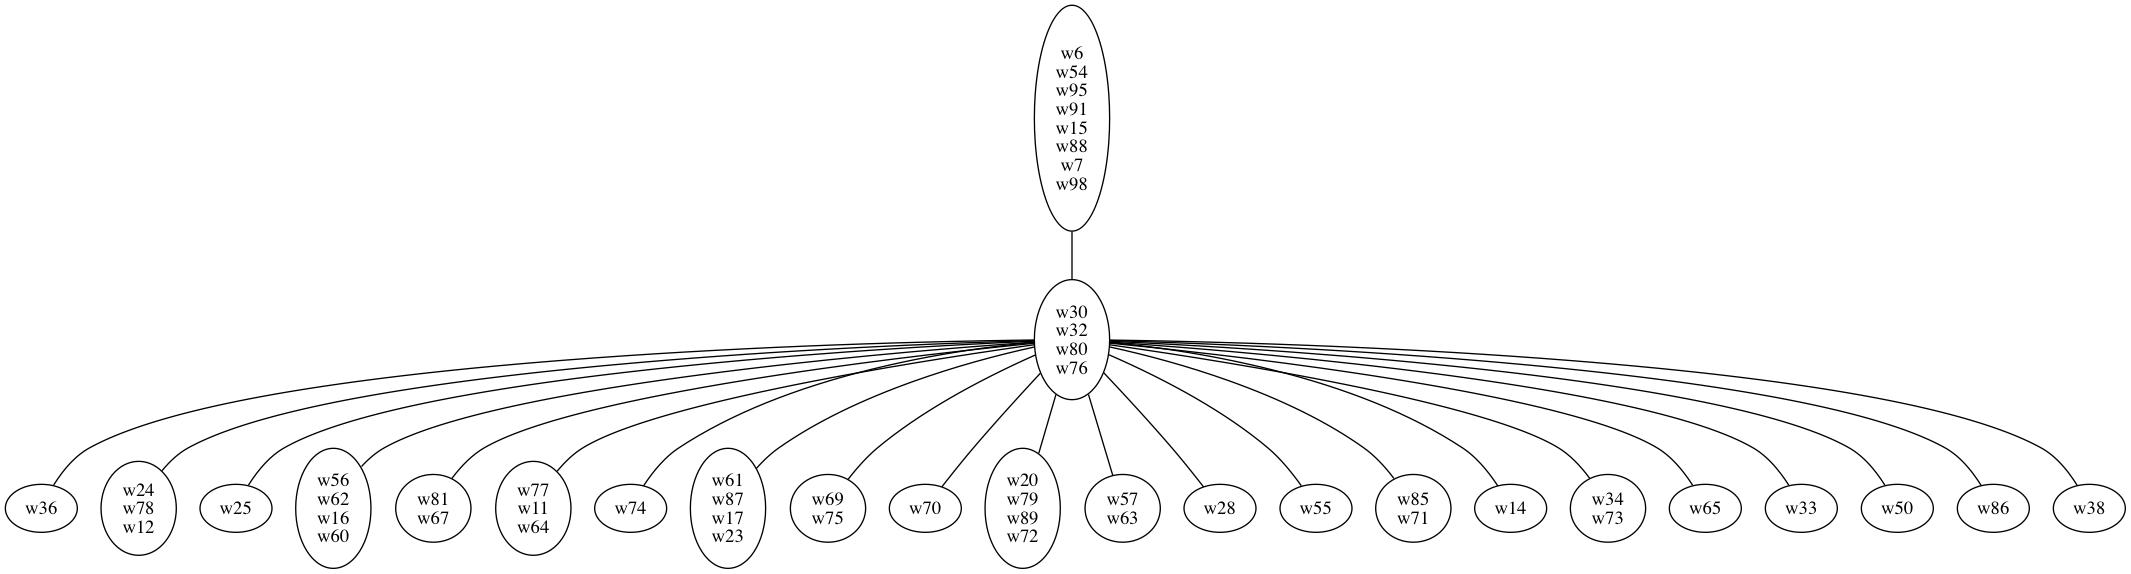
\includegraphics[width=0.9\textwidth]{sim.png}
\caption{ hLDA with three level hierarchy}
\label{fig:h1}
\end{figure}


\begin{figure}
\center
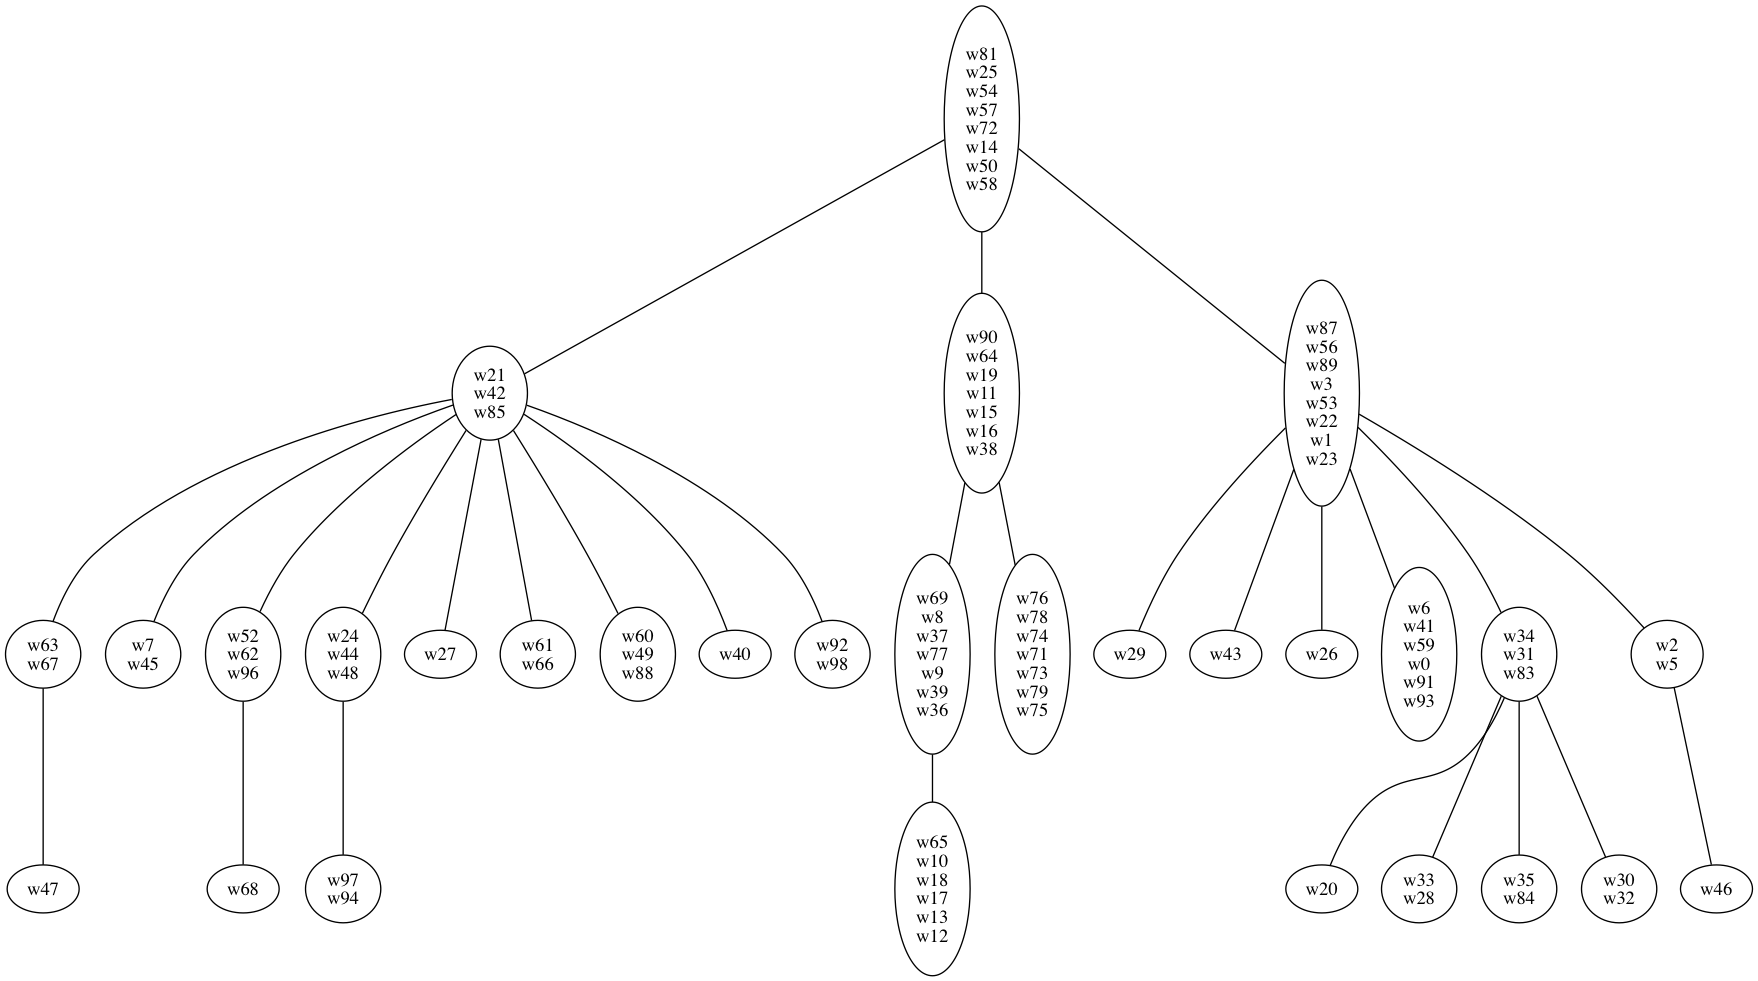
\includegraphics[width=0.9\textwidth]{sim2.png}
\caption{ hLDA with four level hierarchy}
\label{fig:h1}
\end{figure}


\newpage
\bibliographystyle{plain}
\bibliography{citation}

\end{document}